\documentclass[11pt,a4paper]{article}

\usepackage[T1]{fontenc}
\usepackage[utf8]{inputenc}
\usepackage{lmodern}
\usepackage[a4paper,margin=2.1cm]{geometry}
\usepackage{xcolor}
\usepackage{hyperref}
\usepackage{pdfpages}

\definecolor{ink}{HTML}{172033}
\definecolor{accent}{HTML}{087F8C}
\definecolor{soft}{HTML}{EDF8F8}
\definecolor{muted}{HTML}{5D6778}

\hypersetup{
  colorlinks=true,
  linkcolor=accent,
  urlcolor=accent,
  pdftitle={Recueil des exercices MAT101},
  pdfauthor={Université Grenoble Alpes - sélection et index Kieran McShane},
  pdfsubject={103 exercices de mathématiques de niveau L1}
}

\pagestyle{empty}
\setlength{\parindent}{0pt}

\newcommand{\chapterlink}[4]{%
  \par\medskip
  \colorbox{soft}{%
    \parbox{\dimexpr\linewidth-2\fboxsep\relax}{%
      \vspace{0.25em}
      \textbf{\hyperref[#1]{#2}}\hfill
      \textcolor{accent}{\textbf{#3 exercices}}\\[0.2em]
      \textcolor{muted}{#4}
      \vspace{0.25em}
    }%
  }%
}

\begin{document}
\pagenumbering{roman}

\begin{titlepage}
  \color{ink}
  \vspace*{2.2cm}

  {\Large UNIVERSITÉ GRENOBLE ALPES\par}
  \vspace{1.4cm}

  {\Huge\bfseries Recueil des exercices MAT101\par}
  \vspace{0.55cm}
  {\LARGE Langage mathématique, algèbre et géométrie élémentaires\par}

  \vspace{1.6cm}
  \colorbox{soft}{%
    \parbox{\dimexpr\linewidth-2\fboxsep\relax}{%
      \centering
      \vspace{0.8em}
      {\Huge\color{accent}\bfseries 103 exercices}\\[0.45em]
      {\large Niveau L1 - énoncés originaux préservés}
      \vspace{0.8em}
    }%
  }

  \vfill
  {\large
    20 exercices sur les nombres complexes\\[0.25em]
    35 exercices sur les ensembles et le langage mathématique\\[0.25em]
    31 exercices sur les fonctions et le dénombrement\\[0.25em]
    17 exercices sur les limites de suites
  \par}

  \vfill
  {\small
    Extraits du polycopié collectif MAT101 de l'Université Grenoble Alpes,
    édition du 13 septembre 2022. Les pages d'énoncés sont reproduites sans
    retranscription afin de préserver les formules, la numérotation et les
    niveaux de difficulté.
  \par}
\end{titlepage}
\setcounter{page}{2}

\phantomsection
\section*{Sommaire}
\addcontentsline{toc}{section}{Sommaire}

Ce recueil rassemble uniquement les pages d'exercices du polycopié MAT101.
Les liens ci-dessous conduisent directement aux quatre parties.

\chapterlink{complexes}{1. Nombres complexes}{20}
  {Exercices 1.1 à 1.20 - pages originales 30 à 35}

\chapterlink{ensembles}{2. Ensembles et langage mathématique}{35}
  {Exercices 2.1 à 2.35 - pages originales 61 à 70}

\chapterlink{fonctions}{3. Fonctions et dénombrement}{31}
  {Exercices 3.1 à 3.31 - pages originales 93 à 103}

\chapterlink{limites}{4. Limites de suites}{17}
  {Exercices 4.1 à 4.17 - pages originales 116 à 120}

\vfill
\textbf{Lecture des niveaux.}
Les exercices marqués (*) vérifient les notions essentielles ; les exercices
(**) correspondent au niveau généralement attendu à l'examen ; les exercices
(***) proposent un approfondissement.

\medskip
\textbf{Source.}
Polycopié collectif MAT101, Université Grenoble Alpes, responsable de l'édition
citée : Raphaël Rossignol. Une version institutionnelle du polycopié est
disponible sur le site de l'Institut Fourier.

\clearpage
\pagenumbering{arabic}
\phantomsection\label{complexes}
\pdfbookmark[1]{1. Nombres complexes}{bookmark-complexes}
\includepdf[pages=30-35]{mat_101_20220913.pdf}

\phantomsection\label{ensembles}
\pdfbookmark[1]{2. Ensembles et langage mathématique}{bookmark-ensembles}
\includepdf[pages=61-70]{mat_101_20220913.pdf}

\phantomsection\label{fonctions}
\pdfbookmark[1]{3. Fonctions et dénombrement}{bookmark-fonctions}
\includepdf[pages=93-103]{mat_101_20220913.pdf}

\phantomsection\label{limites}
\pdfbookmark[1]{4. Limites de suites}{bookmark-limites}
\includepdf[pages=116-120]{mat_101_20220913.pdf}

\end{document}
